%% ============================================================
%% 分片 22：原文第 9 节「't Hooft And Hecke Operators」（原文 glshort.tex 起于第 6755 行）
%% 由 tools/harvmac2tex.py 从 arXiv 源码（hep-th/0604151v3）自动生成。
%% 只译英文散文；公式、编号、\label、\cite 一律不改。
%% ============================================================

\section{'t Hooft 算子与 Hecke 算子}
\label{sec:thooftheckeop}

\begin{keytakeaways}
  \begin{itemize}[leftmargin=1.4em,itemsep=2pt,topsep=2pt]
    \item \textbf{物理图像}：在 $\Psi=0$（即令 $t=1$、$\theta=0$）处，四维拓扑场论在二维约化为靶空间为 Hitchin 模空间 $\MH$、复结构为 $K$ 的 $A$-模型；支撑在 $\Bbb{R}\times p$ 上的静态 't Hooft 圈算子在二维就是该 $A$-模型中的缺陷，它靠制造指定的奇点来起作用。
    \item \textbf{数学工具}：$A$-模型的经典位形是全纯映射，其态空间的经典近似是常值映射空间的上同调（在 Floer 理论中即两个拉格朗日子流形之交的上同调，需按 Maslov 指标移动维数）；四维侧用消灭定理与 Bogomolny 方程 $F=\star D\phi_0$（BPS 单极子方程）把问题化到三维。
    \item \textbf{关键结论}：静态 't Hooft 算子实现 $G$-丛的 Hecke 变换。局部写 $E=\oplus_i{\cal L}_i$ 后，算子 $T({}^L w)$ 的作用恰为 ${\cal L}_i\to{\cal L}_i\otimes{\cal O}(p_0)^{m_i}$，这正是几何 Langlands 纲领中 Hecke 修正的标准数学定义，因此 't Hooft 算子对应 Hecke 算子。
    \item \textbf{边界与展望}：本节只处理普通 Bogomolny 方程；几何 Langlands 的实际应用需要放宽时间反演对称性，改用复化（扩展）的 Bogomolny 方程，此时 't Hooft 算子给出 Hitchin 对 $(E,\varphi)$ 的 Hecke 变换，见第~\ref{sec:extbog}~节。
  \end{itemize}
\end{keytakeaways}

本节的目的是开始研究在 $\Psi=0$ 处出现的超对称 't Hooft 算子；这个取值通过令 $t=1$、$\theta=0$ 达到。主要结果将是证明：'t Hooft 算子对应于几何 Langlands 纲领中的 Hecke 算子。

我们将主要考虑静态 't Hooft 算子。于是四维流形取为 $M=\Bbb{R}\times W$，其中 $W$ 是某个三维流形；而 't Hooft 线算子将支撑在形如 $\Bbb{R}\times p$ 的一维流形上，其中 $p\in W$ 是某个点。正如我们在第~\ref{sec:loopop}~节讨论过的，这类线“算子”并不是通常意义下作用在某个预先存在的向量空间上的算子；相反，它们必须被纳入物理的、超对称的态空间的定义之中。

我们的 $\Psi=0$ 处四维拓扑场论在二维约化为靶空间为 $\MH$、复结构为 $K$ 的 $A$-模型。所以先回顾 $A$-模型的一些事实。一般地，在靶空间为 $X$ 的二维 $A$-模型中，超对称经典场位形是全纯映射 $\Phi:\Sigma\to X$。此外，超对称态空间的第一近似是 $\Sigma=\Bbb{R}\times I$ 上不依赖时间的超对称经典场所构成空间的上同调，其中 $I$ 是一个区间。超对称场就是全纯映射 $\Phi:\Sigma\to X$。但一个既全纯又不依赖时间的映射必为常值映射。所以在 $A$-模型中，物理态空间的经典近似就是满足边界条件的、到 $X$ 的常值映射所构成空间的上同调。例如在 Floer 理论中，人们取这样的边界条件：$\Bbb{R}\times I$ 的两个边界分支分别映入两个指定的拉格朗日子流形 $N,N'\subset X$。满足这些边界条件的常值映射必须把 $\Sigma$ 映入交 $N\cap N'$，于是超对称态空间的经典近似就是 $N\cap N'$ 的上同调。（必须移动上同调类的维数或鬼数（ghost number），以计入真空中被填满的费米子态数目。数学上，这个移动涉及 Maslov 指标。）

一般地，这个经典交会受到瞬子修正；对瞬子的研究正是 Floer 理论的主要内容。但我们将会看到，对于我们考虑的膜，$\Psi=0$ 处的 $A$-模型没有瞬子修正；超对称位形全都不依赖时间。

\par\medskip{\it 约化到二维}

为了约化到 $\Bbb{R}\times I$ 上的二维模型，我们特殊化迄今一直取为 $M=\Bbb{R}\times W$ 的四维流形：取 $W=I\times C$，其中 $C$ 是黎曼面，$I$ 是一个区间，并在其两端取由膜的选择所定义的边界条件。总起来说，我们在 $M=\Bbb{R}\times I\times C$ 上工作。超对称条件与第~\ref{sec:familya}~节中所见的相同：
% 式 (9.1)
\setcounter{equation}{0}
\begin{equation}\label{eq:oops}
\begin{aligned}(F-\phi\wedge\phi+tD\phi)^+ & = 0 \\
                      (F-\phi\wedge\phi-t^{-1}D\phi)^-& = 0 \\
                      D^* \phi & = 0.\\\end{aligned}
\end{equation}

在 $t=1$（研究 't Hooft 算子时我们通常作此假设）时，\eqref{eq:oops}\ 的前两个方程可写为 $F-\phi\wedge \phi+\star D\phi=0$。用复联络 $\CA=A+i\phi$ 及其曲率 $\CF=d\CA+\CA\wedge\CA$ 表示，这等价于 % 式 (9.2)
\setcounter{equation}{1}
\begin{equation}\label{eq:nops}
{\cal F}+i\star\bar\CF=0.
\end{equation}

在没有 't Hooft 圈、并取适当边界条件时，与第~\ref{sec:vanishing}~节类似的消灭定理表明：这些方程在 $M=\Bbb{R}\times I\times C$ 上的解是从 $C$ 拉回的，并且来自 $\Sigma=\Bbb{R}\times I$ 到 $\MH$ 的常值映射。这是四维拓扑场论约化为二维 sigma 模型的一部分。

\begin{figure}[htbp]
\centering
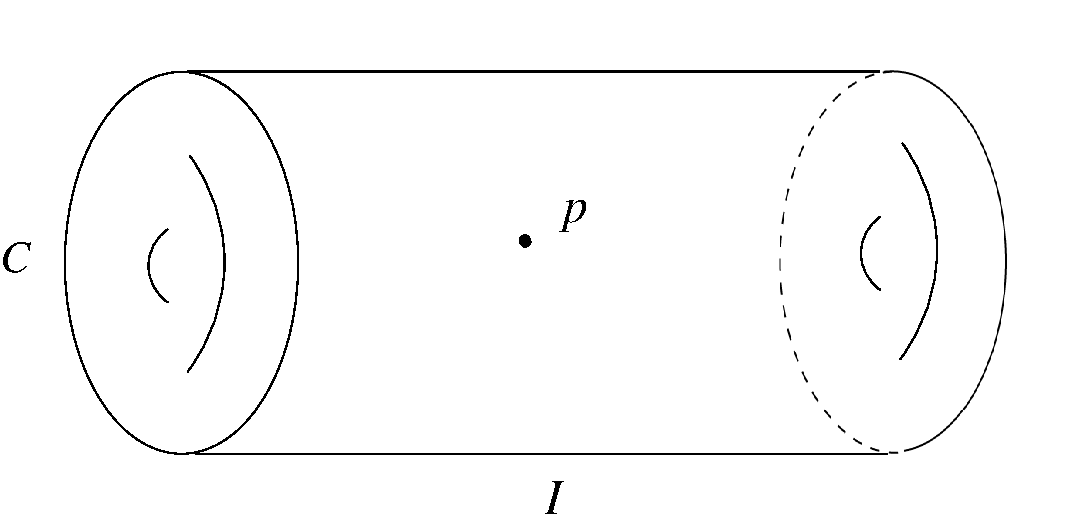
\includegraphics[width=0.75\linewidth]{figures/gla7-1.png}
\caption{插在 $I\times C$ 中点 $p=y\times p_0$ 处的静态 't Hooft 线。在该点附近，Bogomolny 方程的解具有指定的奇点。（原文 Fig.~12）}
\label{fig:botampo}
\end{figure}

把 't Hooft 线包含进来后，事情变得更复杂（\botampo）。如我们从第~\ref{sec:tophooft}~节回忆的那样，'t Hooft 算子在经典场位形中制造指定的奇点。对于支撑在直线 $\Bbb{R}\times p$ 上的 't Hooft 算子（其中 $p\in I\times C$），奇点将妨碍我们证明解是从 $C$ 拉回的。但对某些边界条件，仍有一个较弱的消灭结果成立：\eqref{eq:oops}\ 的相关解不依赖时间，即在对 $\Bbb{R}$ 的平移下不变。

为解释这一点，回忆一下：从几何 Langlands 对偶的观点看，最重要的 $A$-膜是 type ${\CMF}$ 的膜，它们支撑在 Hitchin 纤维化的一个纤维上，并带秩 1 的平坦 Chan-Paton 丛。它们是零膜的 $S$-对偶，因此预期是磁特征膜。正如第~\ref{sec:mhbranes}~节所解释的，它们是 $(B,A,A)$ 型膜，即相应的边界条件与两个线性无关的拓扑超荷相容，而这两个超荷的适当线性组合生成复结构 $I$ 中 $B$-模型的拓扑超对称，以及复结构 $J$ 和 $K$ 中 $A$-模型的拓扑超对称。

当我们考虑具有 $(B,A,A)$ 边界条件并插入 't Hooft 算子的 BRST 不变场位形时，可以区分两类位形：保持两个费米对称性的位形，以及只保持复结构 $K$ 中 $A$-型超对称的位形。在后一情形，破缺的超对称产生一个额外的费米零模；由于它由一个对称性生成，不会被量子修正消除，从而阻止这类瞬子对任何拓扑可观测量作出贡献。（也可能存在其他费米零模，其存在性并不来自费米对称性。）因此，感兴趣的贡献只来自同时保持两个超对称的瞬子。

事实上，具备所需性质的瞬子不依赖时间。从 sigma 模型即可猜到此点，因为复结构 $I$ 中的 $B$-模型没有非平凡瞬子。在 $\Bbb{R}\times I\times C$ 上完整扭化超对称规范场论的框架中，即使存在静态 't Hooft 算子，该结论也成立。最一般的证明涉及 moment map 论证，将另文给出 \cite{ref26}。这里我们概述另一个论证，它对最重要的 $(B,A,A)$-膜（例如 ${\CMF}$ 型膜）已经足够。

首先我们需要一个关于 $\phi_1$ 的消灭定理，$\phi_1$ 是 $\phi$ 在 $M=\Bbb{R}\times I\times C$ 的 $I$ 方向上的分量。在任何一个经典瞬子解中，$\phi_1$ 满足它自己的二阶 Euler-Lagrange 方程，这些方程可由经典作用量 \eqref{eq:nuseful}\ 推出，其形式为 % [WARN] 公式 \eqn\eqref{eq:zungo} 无编号或重复
\begin{equation*}
\tag*{(9.3)}
-D_\mu
D^\mu\phi_1+[\phi_\mu,[\phi_1,\phi^\mu]]=0.
\end{equation*}
 我们假设 $\phi_1$ 在每个膜上满足 Dirichlet 或 Neumann 边界条件；对最重要的那些膜这是成立的。用 $\phi_1$ 乘该方程、取迹并在时空上积分，得到
% 式 (9.4)
\setcounter{equation}{3}
\begin{equation}\label{eq:wungo}
\int d^4x\ \Tr\left( D_\mu\phi_1
D^\mu\phi_1+[\phi_1,\phi_\mu][\phi_1,\phi^\mu]\right)=0.
\end{equation}

分部积分不产生边界项，因为已假定了边界条件；而且 't Hooft 算子带来的奇点也不成问题，因为 $\phi_1$ 在静态 't Hooft 算子附近非奇异。由于被积式是负定的，上述恒等式蕴含 $D_\mu\phi_1=[\phi_\mu,\phi_1]=0$，从而在解不可约的情形下 $\phi_1=0$。

在这个论证中，我们默认分部积分在遥远的过去或未来不产生边界项。我们并不能先验地知道方程的超对称解不依赖时间。然而，我们至少假设所需的解在遥远的过去或未来趋近于不依赖时间的“真空”解。先对时间无关的情形运行上一段的论证，便可得知每个真空中 $\phi_1=0$。于是，由于 $W$ 紧，$\phi$ 在遥远的过去或未来以指数速度趋于 0。因此，上一段用来证明处处 $\phi_1=0$ 的分部积分中没有边界项。

现在我们要证明：一个既具有复结构 $J$ 中又具有复结构 $K$ 中 $A$-模型的拓扑超对称、并且满足 $\phi_1=0$ 的场，实际上不依赖时间。复结构 $K$ 中 $A$-模型的超对称方程就是 $t=1$ 时的方程 \eqref{eq:oops}；复结构 $J$ 中 $A$-模型的方程则由此作一个 ${\cal U}_1$ 变换 $\varphi\to i\varphi$ 得到。把 $M=\Bbb{R}\times I\times C$ 上合并后的方程组写出来，并证明若再加上 $\phi_1=0$，它们便蕴含场在规范变换下不依赖时间，这是一个小练习。

不依赖时间的超对称场可以在 $M=\Bbb{R}\times W$ 连同静态 Wilson 线的更一般框架中方便地分析（不必特殊化到 $W=I\times C$），尽管我们关于所有相关超对称场都不依赖时间的论证在这种一般性下并不成立。当特殊化到 $M=\Bbb{R}\times W$ 时，还有时间反演不变性这一额外对称性 ${\EUT}$，它作用为 $s\to -s$，其中 $s$ 是 $\Bbb{R}$ 上的“时间”坐标；${\EUT}$ 在 $W$ 上平凡作用，并把 $(A,\phi)\to ({\EUT}^*A,-{\EUT}^*\phi)$。（这是第~\ref{sec:canonpar}~节末尾讨论的定向反转对称性的一个例子。）$\phi$ 的符号改变是必要的，因为 ${\EUT}$ 反转向 \eqref{eq:nops} 中 Hodge $\star$ 算子的符号。

因此，我们可以一致地只考虑既不依赖时间又 ${\EUT}$ 不变的解。在这样的解中，$G$-丛 $E$ 与联络 $A$ 是从 $W$ 拉回的。此外，$\phi$ 取形式 $\phi_0\,ds$，其中 $\phi_0$ 是 $W$ 上取值于 ${\rm ad}(E)$ 的零形式。方程约化为
% 式 (9.5)
\setcounter{equation}{4}
\begin{equation}\label{eq:bogeq}
F=\star D\phi_0.
\end{equation}
 我们的定向约定使四维中 $\star(dx^0\wedge dx^1)=dx^2\wedge dx^3$，三维中 $\star(dx^1)=dx^2\wedge dx^3$。方程 \eqref{eq:bogeq}\ 是标准的 Bogomolny 方程 \cite{ref105}，描述超对称或 BPS 单极子\footnote{这个名称反映了这样一个事实：基本的超对称单极子解也在 \cite{ref106} 中作为二阶 Yang-Mills-Higgs 方程的解被发现。}，并且已得到广泛研究，例如 
\cite{ref107,ref108,ref109}。得到 Bogomolny 方程的更熟悉的方式，是寻找 $\Bbb{R}^4$ 上沿某一方向平移不变的 Yang-Mills 瞬子方程的解。

本节中，我们将首先在普通 Bogomolny 方程 \eqref{eq:bogeq} 的框架下分析静态 't Hooft 算子。我们将证明它们实现 $G$-丛的 Hecke 变换，也就是几何 Langlands 纲领中通常定义的 Hecke 变换（Hecke transformation）。这将涉及研究带有由 't Hooft 算子造成的点奇点的 BPS 单极子解。Bogomolny 方程的这种奇异解最早由 Kronheimer 在未发表的工作 \cite{ref110} 中研究过。它们可以作为更大规范群的光滑单极子解的极限出现 
\cite{ref111,ref112,ref113,ref114}，也可来自某些弦论膜位形 \cite{ref115}，后者启发了更晚近的研究 
\cite{ref116,ref117,ref118}。然后我们将对 $G$-丛的 Hecke 修正作一个初等的介绍——从数学观点看既不声称新颖、也不声称完备！

在第~\ref{sec:extbog}~节中，我们将推广这一分析，放宽时间反演对称性的假设。我们将会看到，在这种情形下，超对称方程给出 Bogomolny 方程的一种复化或扩展的类似物，它似乎尚未被研究过。在这些扩展方程的框架中，静态 't Hooft 算子通过 Higgs 丛（换言之，Hitchin 对 $(E,\varphi)$）的 Hecke 变换起作用。这种扩展意义上的 Hecke 算子在数学上是自然的，并且此前已被考虑过 
\cite{ref119,ref120}。

几何 Langlands 纲领中的应用实际上依赖于扩展的 Bogomolny 方程与扩展的 Hecke 算子。只有当边界条件（即膜的选择）保证 Higgs 场 $\varphi$ 消失时，我们才能退回到普通的 Bogomolny 方程与 Hecke 算子。典型应用并非这种情形。不过，我们从普通的 Bogomolny 方程与 Hecke 算子讲起，并把大部分注意力放在它们上面，因为这种情形更简单，且能展示主要思想。

\begin{yizhu}[原文疑误]
式 (9.4) 下方原文称被积式是“负定的”（negative-definite），译文照原文译作负定。按：$M=\Bbb{R}\times I\times C$ 是黎曼流形，在 $\Tr$ 下 $D_\mu\phi_1D^\mu\phi_1$ 是半正定的，而 $[\phi_1,\phi_\mu][\phi_1,\phi^\mu]$ 的迹也非负（因 $[\phi_1,\phi_\mu]$ 反厄米，其平方取迹为负），故该被积式应为半正定；原文用“负定”多半是沿用了把作用量写成 $-\int\Tr(\cdots)$ 的符号约定。结论 $D_\mu\phi_1=[\phi_\mu,\phi_1]=0$ 不受影响。
\end{yizhu}

\begin{yizhu}[易错点]
$t=1$ 时式 (9.1) 的前两式为何合并为 $F-\phi\wedge\phi+\star D\phi=0$：记 $X=F-\phi\wedge\phi$。四维中 $\star$ 把自对偶 2-形式映为反自对偶、反之亦然，且 $\star^2=1$，故 $X\pm\star D\phi=0$ 的自对偶部分为 $X^+ +(D\phi)^+$、反自对偶部分为 $X^--(D\phi)^-$；而 $(D\phi)^\pm$ 正是 $D\phi$ 的（反）自对偶投影。于是 $X+\star D\phi=0$ 恰好同时等价于 $(X+D\phi)^+=0$ 与 $(X-D\phi)^-=0$，即式 (9.1) 在 $t=1$ 的前两式。按：这一步是后文把超对称条件写成复联络方程 (9.2) 的关键，读 (9.2) 时须记住 $\CA=A+i\phi$ 的虚部就是 Higgs 场（在复结构 $I$ 中）。
\end{yizhu}

\begin{yizhu}[易错点]
式 (9.5) 前后的定向约定：原文取四维 $\star(dx^0\wedge dx^1)=dx^2\wedge dx^3$，三维 $\star(dx^1)=dx^2\wedge dx^3$。这里 $s=x^0$ 是 $\Bbb{R}$ 上坐标，$x^1$ 是 $W$ 上坐标；两个式子的相容性在于 Hodge 星对分解 $M=\Bbb{R}\times W$ 满足 $\star_4(ds\wedge\alpha)=\star_3\alpha$。由于 $\phi=\phi_0\,ds$ 是沿 $ds$ 的 1-形式，$D\phi$ 与 $F$ 都是 2-形式，式 (9.5) 中出现的 $\star$ 实际是 $W$ 上的三维 $\star$（作用在 $W$ 的 2-形式上）。按：若把这里的 $\star$ 误当成四维 $\star$，会多出 $ds$ 因子，方程 (9.5) 就不成立了。
\end{yizhu}

\begin{yizhu}[易错点]
时间反演 ${\EUT}$ 为何要令 $\phi$ 变号：$s\to -s$ 反转 $M=\Bbb{R}\times W$ 的定向，从而 $\star\to -\star$，方程 (9.2) ${\cal F}+i\star\bar\CF=0$ 不再保持原形。若同时把 $\CA=A+i\phi$ 换成其复共轭 $\bar\CA=A-i\phi$（即 $\phi\to-\phi$），则 ${\cal F}\leftrightarrow\bar\CF$，方程化为原方程的共轭式，仍然成立。按：原文把这条变换放在“定向反转对称性”的一般框架下（第~\ref{sec:canonpar}~节末），$\phi$ 是 1-形式，其时间分量在此变换下的行为正是 $\phi_0\,ds$ 中 $ds$ 被反转、再整体补一个负号的结果；后文推 (9.5) 时用的就是这个不变性。
\end{yizhu}

\begin{yizhu}[物理图像]
为什么 $\Psi=0$ 处“没有瞬子修正”、超对称位形都不依赖时间：在 $(B,A,A)$ 型边界条件下，$B$-模型（复结构 $I$）部分没有非平凡瞬子（$I$ 中 $B$-模型的态空间经典近似即常值映射上同调），而 $A$-模型（复结构 $J,K$）部分的瞬子若只保持一个超荷，就会产生不被量子修正消除的费米零模，从而对拓扑可观测量无贡献；因此有贡献的瞬子必须同时保持两个超荷，而这类位形可证不依赖时间。参见 Witten 2008 综述关于 B-模型/A-模型与 Hitchin 纤维化的讨论。按：这正是本节能把四维问题约化为三维 Bogomolny 方程的依据；一旦放宽时间反演假设（下节），就会出现扩展 Bogomolny 方程。
\end{yizhu}

\begin{yizhu}[易错点]
本片沿用的 harvmac 记号不要展开或改名：${\CMF}$ 是 $\mathbf{F}$（Hitchin 纤维化的典型纤维），不是普通的 $\cal F$；$\botampo$、$\otampo$、$\notampo$ 分别展开为 “fig.~12/13/14”（原文图号，见 macros.tex），与 \verb|\ref| 不同，不要替换成 \verb|\ref{fig:...}|；${\EUT}$ 是时间反演对称性、${\EUN}$ 是 $\cal N$。此外“鬼数（ghost number）”的移动就是按填入的费米子态数平移上同调的次数，与 Maslov 指标在 Floer 理论中的作用相同。
\end{yizhu}
